% !TEX root = main.tex
\chapter{Introduction}
\label{introchap}

\section{Background}
Pin-point landing has been of significant interest for a variety of applications. These include safely landing scientific payloads and humans on other planets, returning them back to Earth, and reusable launch vehicles (RLVs). The ability to soft-land a rocket is fundamentally disruptive to the launch industry and has already showed promise in reducing the cost of getting to space \cite{jones2018recent}. For planetary exploration, it will be a requirement to land near a site of scientific interest, base, or refueling stations. It is apparent that having a robust and reliable powered descent guidance routine will be a necessity for future space transport infrastructure.

Every pinpoint landing problem begins with an entry phase where the vehicle descends through an atmosphere to a point where the landing regime begins. Many Mars entry, descent, and landing schemes enter the atmosphere and decelerate via an ablative shield and supersonic parachutes. The parachute is then cut away to allow powered descent to occur. With atmospheric qualities being non-deterministic, the position in which the descent phase must begin is uncertain. Therefore, landing algorithms which maximize the divert capability of the vehicle by minimizing the fuel consumption of the final landing time are of interest. Powered descent guidance is the generation of a fuel-optimal trajectory and/or input sequence that takes the vehicle from some initial state condition to a prescribed final state in a uniform gravitational field with standard vehicle given thrust magnitude and direction constraints in finite time. Figure \ref{fig:intro} shows an example of an RLV in a return-to-launch-site maneuver (RTLS).

The convex optimization framework is exploited because it is amenable to real-time, on-board implementation and has guaranteed convergence properties with deterministic criteria. The convex programming algorithm to solve powered descent guidance presented herein has non-convex controls constraints and will be posed as a finite-dimensional second-order cone program (SOCP). SOCPs have low complexity and can be solved in polynomial time \cite{boyd2004convex}.

This thesis focuses on the implementation and development of a 6 degree-of-freedom (DoF) guidance algorithm that solves the non-convex nonlinear powered descent guidance (PDG) problem. A method called successive convexification or SCvx is employed. In this method, the algorithm is initialized with a reference trajectory, then linearized and discretized as an SOCP problem. The problem is then structured as an iterative solution process where the current problem is linearized about the previous trajectory. This is done in such a way that the solution satisfies the original nonlinear dynamics, non-convex constraints, and other state and control constraints. 
\begin{figure}[!htbp] 
  \centering
  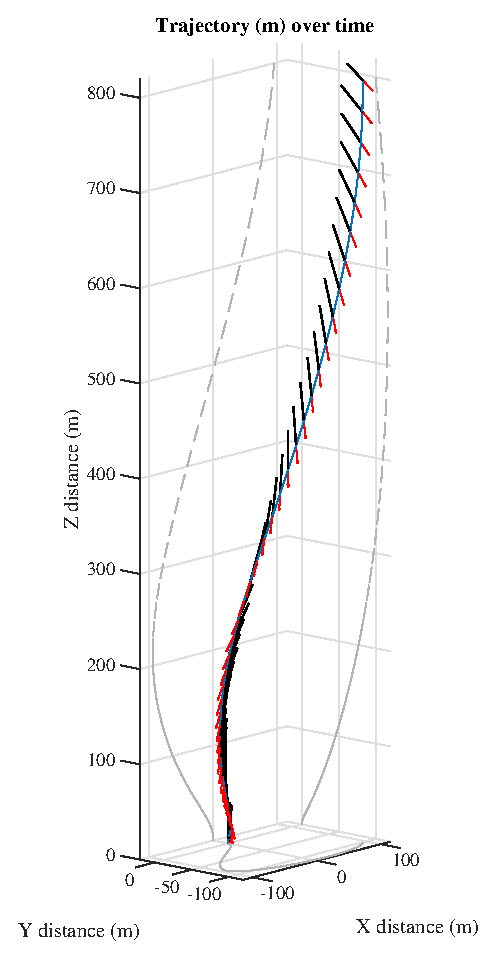
\includegraphics[width=0.25\textwidth]{figs/3dtraj_intro.eps}
  \caption{Landing Trajectory Example}
  \label{fig:intro}
 \end{figure}	



\section{Motivation}
Autonomous optimal guidance strategies enable vehicle recovery from a wider range disturbances accrued from the entry and descent process. This allows the vehicle to optimally maximize the divert and transport capability after dispersions, increasing the probability of safe landing and mission success. The value of these strategies is apparent in the efforts and successes of current commercial space companies which land and reuse their space launch vehicles. The work presented herein has a number of desirable traits which make it amenable to implementation in this context. To sufficiently motivate and further this discussion, let us discuss what factors are important in the selection of a flight guidance algorithm.



\addtocontents{toc}{\protect\setcounter{tocdepth}{1}}
\subsection{Attributes of a Good Guidance Algorithm}
\addtocontents{toc}{\protect\setcounter{tocdepth}{2}}
Nominally, the guidance algorithm must be computationally tractable. These routines run at slower rates than the control and could be computed at the beginning of each phase or run continuously, correcting for large changes in the system or environment.
This is one of the main reasons guidance tends to be run ``offline,'' or not during flight, and stored in look up tables (LUTs). This may also be called ``implicit'' guidance. These are simply stored solutions for the flight computer to use a later time. Sophisticated guidance algorithms that have a full understanding of the problem at hand tend to be quite intensive, therefore it can be beneficial to the engineer to find fast and simple solution mechanisms.

A guidance algorithm must be tractable not only for speed, but also to reduce resource congestion. Other processes, namely the navigation and control routines, also require compute power and should not be throttled. Real-time operating systems have strict schedulers where each task is guaranteed to run to completion in finite time. If a deadline is unable to be met, a priority inversion system is put in place to pause one task and move on to another, for single-threaded operations. Nominally, no algorithm should be so intensive such that it steals resources from other required computational subsystems.

The guidance routine must be accurate to the vehicle, actuator, and environmental dynamics. This will allow the vehicle to enact motions and controls that are consistent with reality. Often the routine is not aware of larger perturbations and accrues significant errors. Even offline LUT methods can fall short here as well, especially when a guidance phase starts with high uncertainty in the initial condition. In this scenario, another outer control loop fixes and applies compensation control effort to re-match the guidance solution; this is now not necessarily an ``optimal'' solution in the same sense as the initially calculated one.

An online method, or one ``explicitly'' computed onboard the flight computer during operation, is a good solution for systems where the initial condition of that phase of flight may disperse widely. If there is high confidence in the navigation solution at the beginning of the guidance routine, but it errs from the nominal point, an online method is attractive. This algorithm can calculate the new, optimal solution for the exact problem at hand. If a rocket is 20 meters from the nominal position, a new state trajectory and input history can be computed on the spot and fed to the control loop which start at that new perturbed condition. A LUT method would require a neighboring optimal control solution to bring it back to the original proposed trajectory which may not guarantee meeting the mission requirements and constraints.

Optimality is also an important consideration in the generation of trajectories and control strategies. If a vehicle requires dynamic constraints or has stringent fuel requirements, a sense of optimality with respect to these key metrics becomes important. For example, these metrics may manifest in a guidance or control law that is accurate to the dynamics, minimizes fuel, or minimizes the final time to the target. If a vehicle must land on the surface of a planet at a specific landing site, a guidance routine which re-targets after significant dispersions and simultaneously minimizes control usage becomes very attractive. Similarly if a vehicle needs to traverse to a nominal state in minimum time and error, but maintain robustness to uncertainties, an optimization based approach is attractive. A trajectory and input sequence that is tailored to these metrics, which are attributed penalty functions and conjoined in the form of a cost function, is then required.

Time ambiguity is another important factor in a good guidance algorithm. Will this algorithm create a control history which meets your objective with free or fixed-final-time? The former means that the terminal time is free and is a solution of the algorithm itself: the vehicle will land on Mars with this trajectory, these inputs, and at exactly 34.5235 seconds from now. The latter first asks you what time you'd like to be there, then produces the required trajectory. The first tends to have a larger sense of optimality than the latter, more restricted second problem, but may be lack robustness close to the terminal state. You could imagine calculating the exact minimum time to achieve a state, but under disturbances being a fraction late and crashing.

A good algorithm must also be inclusive of mission, vehicular, and environmental constraints. Do the crew members enjoy 10g's of acceleration and 45 degrees per second of rotation? Would you like to stay above the ground and never use more fuel than you have? These are important pieces of information to have when making a vital decision about the motion and plan of your space vehicle.

Guarantees of convergence and aforementioned optimality are important for validation and testing of the GN\&C subsystem. What if the algorithm actually never converges in flight, or the output is entirely suboptimal and performs poorly? Having these deterministic guarantees mathematically proven becomes very important when it comes to flying critical hardware and humans.

Fault detection, isolation, and recovery (FDIR) is another critical component. Can the state machine of the vehicle or craft detect a fault and correctly recover? If a system behaves anomalously, for some reason, there must be a robust way to detect this and communicate to other subsystems what has happened. If a guidance routine does not converge, another trajectory or control strategy must be chosen and used quickly before continued off-nominal performance.

The performance with respect to dispersions and sensitive parameters is also important. The algorithm performance in the face of randomness must not degrade significantly. Additionally, the routine should not be overly sensitive to any single parameter. If any algorithm is highly sensitive to a single parameters, say a valve or hydraulic actuation speed variation, it could significantly limit the operational dynamic range of that algorithm. These analyses should be performed rigorously a priori before flight implementation.



% #########################################
\section{Literature Review and Related Research}
Optimal control and guidance strategies are generally split into two categories: indirect and direct methods.
Classical indirect methods are applications of calculus of variations and Pontryagin's Maximum Principle to derive the necessary conditions of optimality, such as adjoint equations and transversality conditions. Although the optimality of the indirect method can be guaranteed, solving the resulted two-point boundary value problem is a difficult task, and good initial guesses of the adjoint variables can be difficult to find or compute.

The direct method does not require explicit derivation of first-order necessary conditions; instead, the original optimal control problem is approximated with a parameter optimization problem and solved using nonlinear programming (NLP) algorithms, such as sequential quadratic programming (SQP) algorithms. Although large-scale problems can be handled due to the development of NLP algorithms, the solution process is still time-consuming for complicated problems and dependent upon good initial guesses. Convex optimization approaches are direct optimization methods, however can be reliably solved in polynomial time \cite{nesterov1994interior}.







\underline{Polynomial Guidance} was famously used on the Apollo lunar lander, first landing men on the moon in 1969. The Apollo guidance computer (AGC) had limited compute capability with the algorithms requiring manual re-targeting and flight by the mission pilot. This algorithm was an analytical solution to a boundary valued problem with a fixed time-to-go \cite{klumpp1974apollo}. The final braking law is represented by a quartic polynomial function which connect the initial and terminal states. This result does not satisfy vehicle thrust constraints, and errors introduced by this law must be compensated for by other calculations. Besides the boundary values, there are no state constraints and no optimality with respect to fuel or time. Although compute power was so limited, all lunar powered descent missions were successful thanks to the polynomial and astronaut guidance. Modified versions of this law are still in the literature with an outer time-of-flight search mechanism to effectively make it a free final time-to-go algorithm as well as adding in fuel optimality \cite{d1997optimal}.

\underline{Powered Explicit Guidance} or PEG is another prevalent guidance routine. This was developed to handle all phases of the Space Shuttle exoatmospheric powered flight and their cutoff constraints \cite{mchenry1979space}. This is a simplified vector form of a linear tangent steering law. It provides robust guidance for situations which vary widely in thrust-to-weight ratios (TWRs). During the second stage of Shuttle ascent, the TWRs range from 1 to 3 with altitude, velocity, flightpath angle, and orbital plane cutoff constraints. The objective of this algorithm is to generate steering and throttle commands such that the cutoff constraints are satisfied in a fuel-efficient manner. This linear tangent scheme is based on an indirect calculus of variations solution to the minimum-fuel ascent trajectory problem. The thrust attitude takes the form of $\lambda_F = \lambda_v + \dot{\lambda}(t - t_\lambda)$ where $\lambda_F$ is the vector defining the thrust direction, $\lambda_v$ is the unit vector in the direction of velocity-to-be-gained, $\dot{\lambda}$ is a vector normal to $\lambda_v$ representing the rate of change of $\lambda_F$. The variable $t$ is continuous time where $t_\lambda$ is a chosen time such that the total velocity change due to thrust is along the vector $\lambda_v$. To satisfy the required cutoff constraints, the algorithm takes the form of a predictor corrector mechanism where $\lambda_v$ is computed such that the terminal velocity constraints are satisfied.

A backwards recursive version of this steering law was developed for the powered descent guidance problem as well. This law minimizes the control required for soft landing but does is not guaranteed to meet all actuator constraints and is naive to the nonlinear dynamics.

\underline{Lossless Convexification} is a method to produce a perfect convex second order cone program (SOCP) sub-problem from an originally non-convex problem statement. It is used for convexifying a non-convex constraint without loosing any precision. This method, championed by Blackmore, Açikmeşe, and Ploen, is at the heart of the G-FOLD landing algorithm \cite{blackmore2010minimum} \cite{accikmecse2011lossless} \cite{acikmese2012g}. The Guidance algorithm for Fuel Optimal Large Diverts, or G-FOLD, is a recent advancement in PDG solutions. It very quickly calculates a 3DoF fuel optimal divert maneuver with free-final-time, inequality and equality constraints on the states and inputs, and losslessly convexifying the lower thrust constraint. Some of these constraints include a glideslope around the target and maximum velocity. The routine solves a lossless convex SOCP problem iteratively with an outer time of flight search loop to find the optimal final time. This was successfully demonstrated in a family of flight experiments on Masten Space landing vehicles \cite{acikmese2013flight} \cite{scharf2014adapt}.

Unfortunately, only a couple types of constraint can be convexified in this fashion, where the remaining nonlinear dynamics are the primary sources of non-convexity. These must be included into the problem statement with another process.

\section{Brief Introduction to Convex Optimization}
A convex optimization problem is one that takes the following form:
\begin{align*}
	\text{minimize} \quad & f_0(x) \\ 
	\text{subject to} \quad & f_i(x) \leq b_i, \ \ i = 1, \cdots, m
\end{align*}
where each of the functions $f_0,...,f_m \ :\mathbb{R}^n \rightarrow \mathbb{R}$ are convex. This means they satisfy the generalized inequality $f_i(\alpha x + \beta y) \leq \alpha f_i(x) + \beta f_i(y) \quad \forall x, y \in \mathbb{R}^n$ where all $\alpha, \beta \in \mathbb{R}$ with $\alpha + \beta = 1,\ \ \forall \alpha,\beta \geq 0$. Many optimization problems are just special cases of this problem, including the general least-squares and linear programming problems. Because many problems can be considered a subset of this framework, using convex optimization is much like using any other optimization tool. If a problem can be identified or formulated as a convex problem, then one should be able to solve it efficiently with available solvers. However, recognizing a convex function can be nontrivial and there exist many tricks for transforming non-convex problems into convex ones. Significant insight into these mathematical tricks for the formulation of convex problems is excellently documented in the Boyd and Vandenberghe text \cite{boyd2004convex}.

\section{On Successive Convexification}
The successive convexification framework (SCvx) is able to quickly solve optimal control problems with nonlinear dynamics and non-convex state and control constraints. It does this by iteratively solving convex optimization sub-problems, obtained by linearizing non-convexities in dynamics and constraints around the previous iteration solution. These sub-problems employ techniques of virtual control (dynamic relaxation), virtual buffer zones, and trust regions to prevent solution artificial infeasibility and artificial unboundedness. This linearization acts as an approximation, but the solution is driven to convergence within the user's tolerances to solve exactly the originally proposed non-convex optimal control problem with local optimality.

For general real-time autonomy tasks where safety and determinism are prioritized, it is often much better to find a locally optimal solution quickly rather than a globally optimal solution slowly. Generally speaking, nonlinear programming tends to be the method of choice for locally optimal solutions. However, their convergence behaviour is dependent upon the initial guess provided to the solver and do not offer bounds on computational effort required for convergence. These facts are at odds with requirements for real-time embedded applications.

One then may turn to convex optimization methods which can be reliably solved in polynomial time \cite{nesterov1994interior}. Sequential convex programming (SCP) offers a way to solve problems with more general nonlinear dynamics and non-convex constraints. While SCP performs well empirically, no general convergence results have been reported. SCvx differs from other SCP approaches in many ways, including proofs for (weak and strong) global convergence and superlinear convergence rate \cite{mao2016successive}.




% #########################################
\section{Statement of Scope}
This thesis describes the nonlinear equations of motion for a space vehicle, poses a guidance problem, and then modifies it such that it is iteratively solvable. This is done by creating a linear time varying version of the dynamics, discretizing it, and convexifying the problem constraints. 

Once this is done, a reference trajectory is generated as a linearization path for SCvx to solve the problem with initially. This is then performed iteratively with the trajectory and input history from the previous run as the linearization path for the next optimization. This is done until convergence is achieved, determined via user given tolerances. The derivation, performance, and analysis of this algorithm are shown herein.











% BELOW THIS LINE ARE TUTORIALS ON THINGS FROM THE TEMPLATE

% \begin{figure}[htbp]
% 	\caption[Cylinder and measurements]{
% 	This diagram of a cylinder and various
% 	measurements and quantities was actually
% 	made using {\bf xfig}, a freeware
% 	drawing program for Unix systems.
% 	Diagrams can be exported directly to PDF
% 	files, the preferred format for
% 	vector graphics.  Vector graphics can
% 	be magnified indefinitely without degradation,
% 	whereas bitmap images (JPG and PNG)
% 	must be pretty high-resolution if you don't
% 	want them looking all pixellated when
% 	magnified.
% 	}
%     \begin{center}
% 	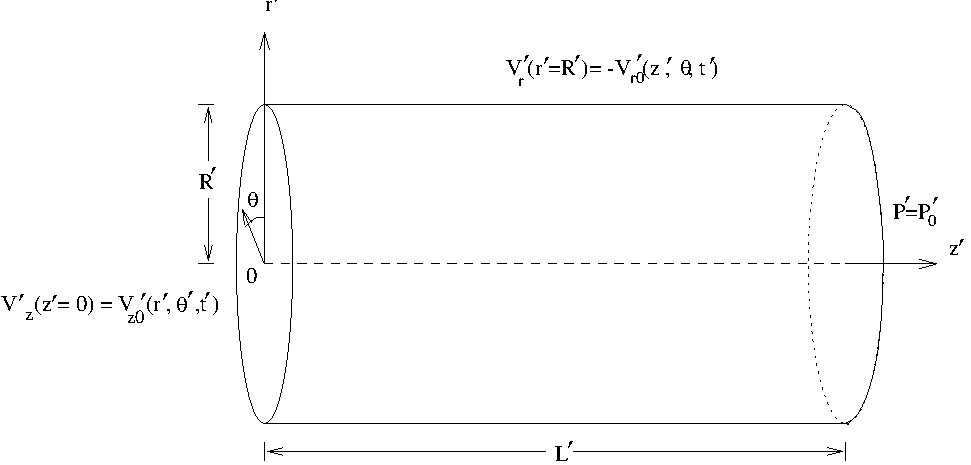
\includegraphics[width=100mm]{figs/cyl.pdf}
%     \end{center}
% \label{xfigDiagram}
% \end{figure}


% \begin{figure}[htbp]
%     \caption[Bitmap images]{
% 	The JPEG bitmap format is great for photos but
% 	crummy for diagrams (including drawings, graphs,
% 	charts) because it can't gracefully handle sharp edges.
% 	Note the same bitmap image below from a PNG file and
% 	from a JPG file; the latter shows characteristic
% 	``ringing'' at sharp edges -- including text!
% 	Seriously, magnify and look closely at the JPG's
% 	awful lines and edges.
% 	Vector-format PDF is the best for diagrams, but
% 	if you must use a bitmap image, let it be PNG.
% 	~ (Left: file {\it drawing.png}.
% 	Right: file {\it drawing.jpg}.)
% 	}
%     \begin{center}
% 	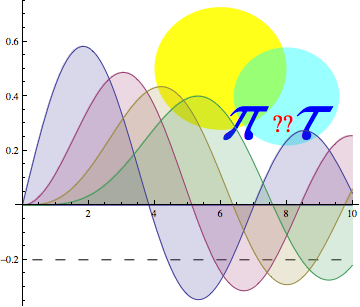
\includegraphics[width=70mm]{figs/drawing.png}
% 	${}^{}$ ~
% 	${}^{}$ ~
% 	${}^{}$
% 	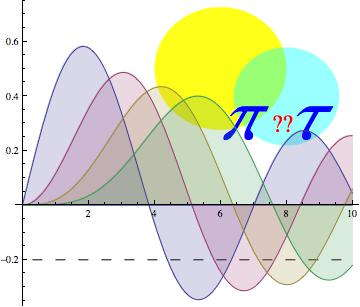
\includegraphics[width=70mm]{figs/drawing.jpg}
%     \end{center}
% \label{bitmapImages}
% \end{figure}



% \section{Lists in {\tt thesis} class}

% In {\tt thesis} class (for Colorado University),
% lists are defined so that nested lists will be
% numbered or marked appropriately.
% First, an itemized (non-enumerated) list
% prefaces each item with a bullet.
% Nested itemized list use asterisks,
% then dashes, then dots.
% These lists are typed between
% the \verb2\begin{itemize}2
% and \verb2\end{itemize}2
% commands.

% \begin{itemize}
%   \item{} This is ``itemized'' item A.
%   \item{} This is ``itemized'' item B.
%   \item{} This is ``itemized'' item C.
%   \begin{itemize}
%     \item{} This is ``itemized'' subitem A.
%     \begin{itemize}
%       \item{} This is ``itemized'' subsubitem A.
%       \begin{itemize}
%         \item{} This is ``itemized'' subsubsubitem A.
%       \end{itemize}
%       \item{} This is ``itemized'' subsubitem B.
%     \end{itemize}
%     \item{} This is ``itemized'' subitem B.
%   \end{itemize}
%   \item{} This is ``itemized'' item D.
% \end{itemize}

% Enumerated lists use the commands
% \verb2\begin{enumerate}2 and
% \verb2\end{enumerate}2,
% and nested enumerations appear like this.

% \begin{enumerate}
%   \item{} This is ``enumerated'' item A.
%   \item{} This is ``enumerated'' item B.
%   \item{} This is ``enumerated'' item C.
%   \begin{enumerate}
%     \item{} This is ``enumerated'' subitem A.
%     \begin{enumerate}
%       \item{} This is ``enumerated'' subsubitem A.
%       \begin{enumerate}
%         \item{} This is ``enumerated'' subsubsubitem A.
%       \end{enumerate}
%       \item{} This is ``enumerated'' subsubitem B.
%     \end{enumerate}
%     \item{} This is ``enumerated'' subitem B.
%   \end{enumerate}
%   \item{} This is ``enumerated'' item D.
% \end{enumerate}


% The work presented
% here\footnote{Footnotes are handled neatly by \LaTeX.}
% is an extension of Lao\cite{lao:thesis}
% and Lao et~al.\cite{lao:paper},
% fictional references that are in the bibliographic
% source file \verb9refs.bib9.

% \begin{table}[htb]
%     \caption[Example of a table with its own footnotes]{
% 	Here is an example of a table with its own footnotes.
% 	Don't use the $\backslash${\tt footnote} macro if you
% 	don't want the footnotes at the bottom of the page.
% 	Also, note that in a thesis the caption goes
% 	\emph{above} a table, unlike figures.
% 	}
%     \begin{center}
%     \begin{tabular}{||l|c|c|c|c||} \hline
% 	& $S$ & $P$ &   $Q^{\ast}$  & $D^{\dagger}$ \\	% footnote symbols!
% 	wave form & (kVA) & (kW) & (kVAr) & (kVAd) \\  \hline \hline
% 	Fig.  \ref{xfigDiagram}a  & 25.48 & 25.00 & -2.82 & 4.03 \\ \hline
% 	Fig.  \ref{xfigDiagram}b  & 25.11 & 18.02 & -9.75 & 14.52 \\ \hline
% 	Table \ref{pdftable}  & 24.98 & 22.26 & 9.19 & 6.64 \\ \hline
% 	Table \ref{powertable}  & 23.48 & 15.00 & 6.59 & 16.82 \\ \hline
% 	Fig.  \ref{pyramid}  & 24.64 & 22.81 & -0.44 & 9.3 \\ \hline
% 	\end{tabular}
%    \\ \rule{0mm}{5mm}
%    ${}^\ast$kVAr means reactive power.		% footnote symbol
% \\ ${}^\dagger$kVAd means distortion power.	% footnote symbol
% \end{center}
% \label{powertable}
% \end{table}


